\documentclass[a4paper]{article}

\usepackage[english,russian]{babel}
\usepackage{hyperref}
\hypersetup{
    colorlinks,
    citecolor=black,
    filecolor=black,
    linkcolor=black,
    urlcolor=blue
}
\usepackage{float}
\usepackage[utf8]{inputenc}
\usepackage[14pt]{extsizes}
\usepackage{graphicx}
\graphicspath{{../misc/}}
\usepackage{setspace,amsmath}
\usepackage[left=20mm, top=15mm, right=15mm, bottom=15mm, nohead, footskip=10mm]{geometry} 

\usepackage[backend=biber]{biblatex}
\addbibresource{lit.bib}

\begin{document} 

\begin{center}
    \hfill \break
    ФЕДЕРАЛЬНОЕ ГОСУДАРСТВЕННОЕ БЮДЖЕТНОЕ ОБРАЗОВАТЕЛЬНОЕ 

    УЧРЕЖДЕНИЕ ВЫСШЕГО ОБРАЗОВАНИЯ

    «МОСКОВСКИЙ ГОСУДАРСТВЕННЫЙ УНИВЕРСИТЕТ

    имени М.В.ЛОМОНОСОВА»

    \hfill \break
    \normalsize{ФИЗИЧЕСКИЙ ФАКУЛЬТЕТ}\\
    \hfill \break
    \normalsize{КАФЕДРА ОБЩЕЙ ФИЗИКИ И МОЛЕКУЛЯРНОЙ ЭЛЕКТРОНИКИ}\\
    \hfill\break
    \hfill \break
    \normalsize{БАКАЛАВРСКАЯ РАБОТА}\\
    \hfill \break
    \large\textbf{«МОДЕЛИРОВАНИЕ РАСПОЗНАВАНИЯ ОБРАЗОВ НА ОСНОВЕ ИСПУЛЬСНЫХ НЕЙРОННЫХ СЕТЕЙ С КОНКУРЕНЦИЕЙ ЛОКАЛЬНЫХ РЕЦЕПТИВНЫХ ПОЛЕЙ»}\\
    \hfill \break

\end{center}

\begin{flushright}

    Выполнил студент:

    406 группа

    Гафни Д.

    $\underset{\text{подпись студента}}{\underline{\hspace{0.3\textwidth}}}$

    \hfill\break

    Научный руководитель:

    Королёва А.В.

    $\underset{\text{подпись научного руководителя}}{\underline{\hspace{0.3\textwidth}}}$
    
    \hfill\break
    
    Научный консультант:

    Дёмин В.А.

    $\underset{\text{подпись научного консультанта}}{\underline{\hspace{0.3\textwidth}}}$

\end{flushright}


Допущена к защите

Зав.кафедрой $\underset{\text{подпись зав.кафедрой}}{\underline{\hspace{0.3\textwidth}}}$
\hfill\break
\hfill\break
\begin{center}

Москва

\hfill\break
2020
\end{center}



\thispagestyle{empty} 

\tableofcontents

\section{Введение}
Импульсные (спайковые) нейронные сети (СНС) являются перспективным нейроморфным алгоритмом, биологически корректно моделируя взаимодействия нейронов мозга. Наибольший интерес СНС представляют для решения задач в реальном времени (принятие решений, распознавание образов), так как могут быть реализованы на специализированном вычислительно- и энергоэффективном мемристорном нейрочипе.  В отличие от формальных нейронных сетей, в спайковых сетях нейроны обмениваются дискретными электрическими сигналами (спайками), существующими во времени. При накоплении потенциала, превышающего определенный порог активации, нейрон сам испускает спайк. Влияние входящих спайков на потенциал нейрона определяется значением веса межнейронной связи. Этим процессам соответствуют аналогичные физические явления в реальных мемристорных сетях.

Стандартные методы обучения весов связей, применяющиеся в формальных нейронных сетях (метод обратного распространения ошибки) не представляется возможным применять к СНС из-за их дискретной и распределенной во времени природы. Таким образом, исследование алгоритмов обучения СНС представляется важной задачей.

\section{Постановка задачи}
В данной работе:

\begin{enumerate}
 \item Изучается влияние обучения связей конкуренции \cite{MaxActiv1} \cite{MaxActiv2} между нейронами на точность распознавания образов в задаче классификации рукописных изображений цифр (MNIST) при обучении без учителя для архитектуры локально соединенной сети (Locally Connected Spiking Neural Network, LCSNN) \cite{saunders2019locally}
 
 \item Проводится сравнение этой архитектуры со сверточной сетью (Convolution Spiking Neural Network, CSNN) и полносвязной сетью (Fully Connected Spiking Neural Network, FCSNN). Обучение производится в соответствии с правилом STDP, используется модель интегрирующих нейронов с утечкой. Все параметры моделей задаются в соответствии с достигаемыми значениями в реальных мемристорах.

\end{enumerate}

\section{Литературный обзор}

\subsection{Мотивация}
\paragraph{Недостатки формальных нейронных сетей}
Современные формальные нейронные сети отлично справляются со многими задачами машинного обучения \cite{pmlr-v28-wan13}. Однако их обучение - трудоемкий процесс, требующий больших вычислительных ресурсов. Обычно обучение ведется на десятках и сотнях тысячах примеров и может занимать месяцы. Как само обучение, так и последующее применение формальных нейросетевых алгоритмов далеки от эффективности. Это связано как с физически раздельным хранением значений весов и активаций нейронов, так и с самими вычислениями, которые носят тензорный характер. Современные процессоры не оптимизированы для подобных вычислений. Вместо них используются GPU - архитектуры, изначально созданные для работы с компьютерной графикой, а потому лучше подходяшие для тензорных вычислений, однако и они не дают желаемого результата. Например, типичное время распознавание лица современными алгоритмами - 200-300 мс.

\paragraph{Плюсы спайковых нейронных сетей}
В отличие от формальных, спайковые нейронные сети:

\begin{itemize}
 \item могут быть реализованы на специализированном сверхэффективном нейроморфном процессоре
 \item биологически корректно моделируют взаимодействия нейронов
\end{itemize}

Ней
*Почему биологическая корректность это хорошо*


\subsection{Спайковая нейронная сеть}
\paragraph{Устройство нейронной сети}
Нейроны там есть всякие спайки
\paragraph{Обучение по правилу STDP}
STDP - Spike Timing Dependent Plasticity - биологически инспирированное правило обучения без учителя.
\begin{equation}
\Delta w =
 \begin{cases}
 A_+ \cdot e^{- \frac{t_{pre} - t_{post}}{\tau_+}}, t_{pre} - t_{post} > 0\\
 A_- \cdot e^{- \frac{t_{pre} - t_{post}}{\tau_-}}, t_{pre} - t_{post} < 0
 \end{cases}
\end{equation}
\begin{figure}
\begin{center}
 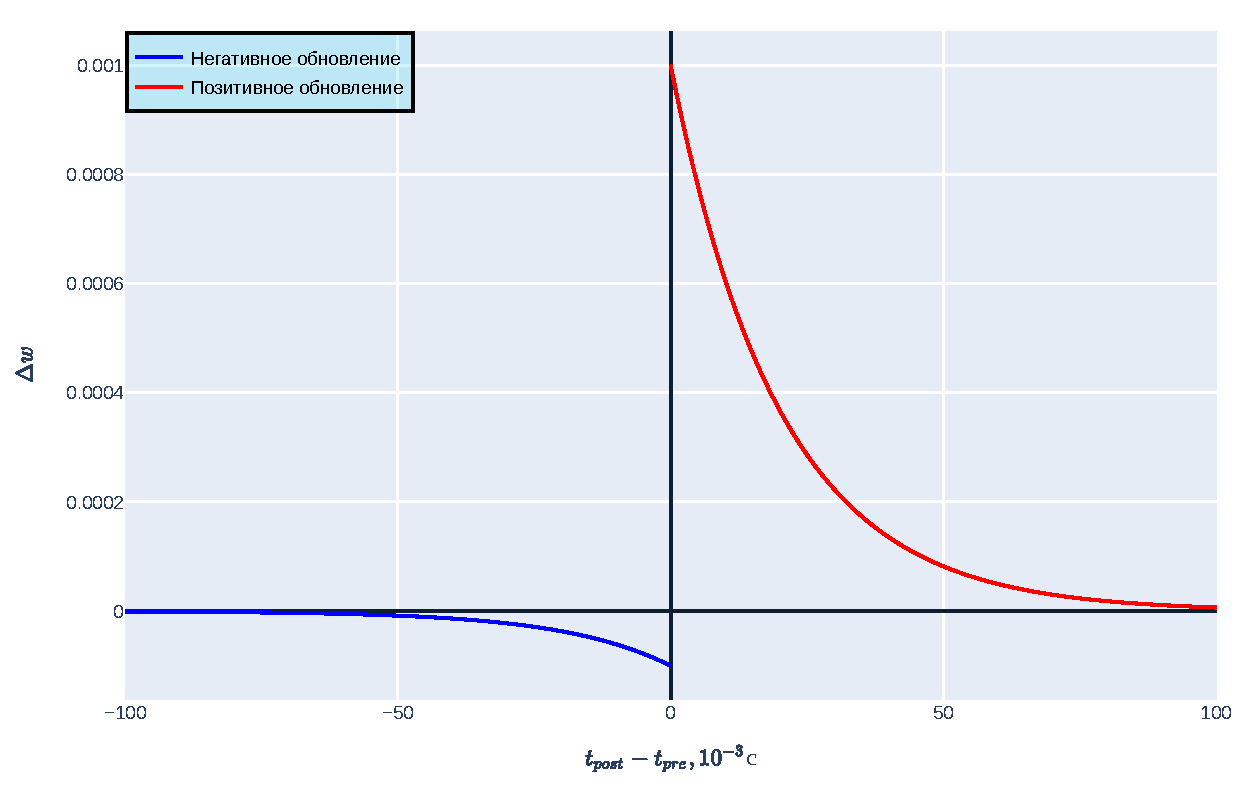
\includegraphics[,
 width=\textwidth,keepaspectratio=true]{STDP.pdf}
 \label{STDP}
 \caption{Правило STDP. График зависимости изменения веса от разности времени регистрации пост- и пре- спайков.}
\end{center}
\end{figure}


\subsection{Локально соединенная архитектура}
Эта нейросетевая архитектура вдохновлена строением зрительной коры мозга. В отличие от сверточной сети, ее нейроны не имеют общих весов, которые потому и называются локальными. На иллюстрации ниже показано строение локально соединенной сети.

\begin{figure}[H]
    \centering
    \def\svgwidth{\columnwidth}
    \input{../misc/LCSNN.pdf_tex}
    \label{LCSNN}
    \caption{Схема архитектуры LCSNN}
\end{figure}

% \begin{figure}
%  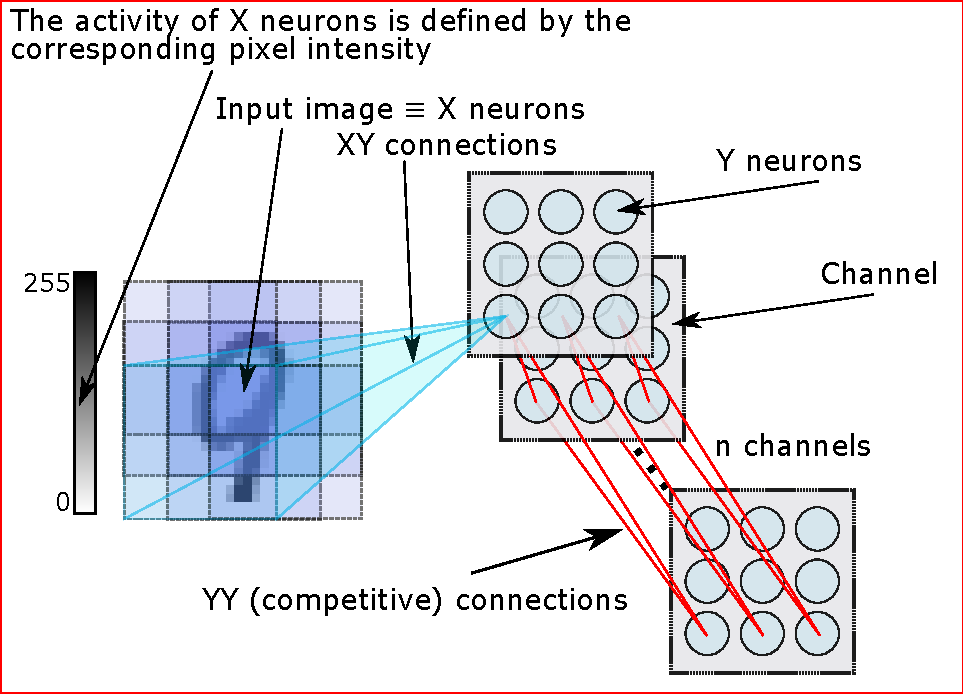
\includegraphics{LCSNN.pdf}
% \end{figure}



Нейроны, имеющие общие рецептивные поля дополнительно соединяются связями конкуренции. Такие связи имеют отрицательные веса, а значит, негативно влияют на активность. Заметим, что нейроны, не имеющие общего рецептивного поля (а значит, реагирующие на разные области изображения) не конкурируют между собой.\\
LCSNN отличаются большой скоростью обучения. Через несколько тысяч итераций точность распознавания выходит на плато насыщения, после чего уже не возрастает.

\begin{center}
\begin{figure}[H]
 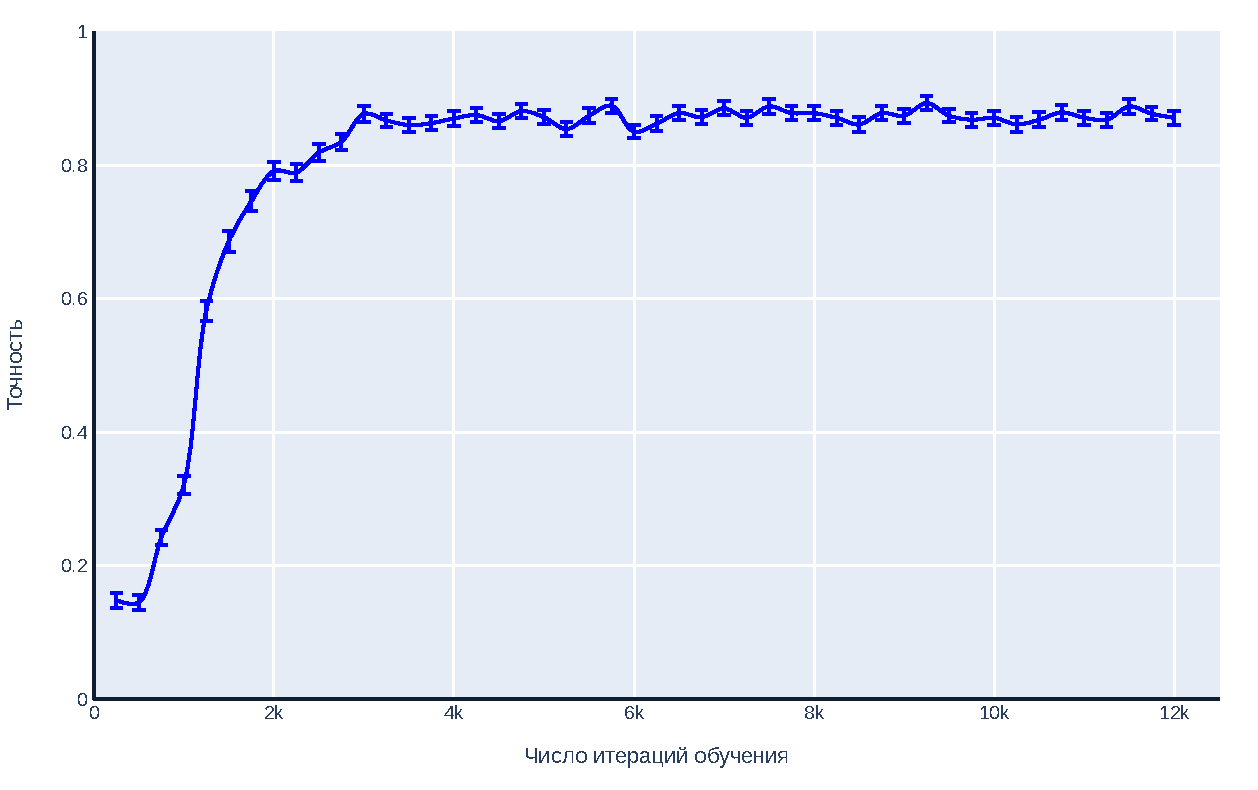
\includegraphics[width=\textwidth,keepaspectratio=true]{acc-n_iter_ru.pdf}
 \caption{Скорость обучения LCSNN}
\end{figure}
\end{center}

\begin{figure}
\begin{center}
 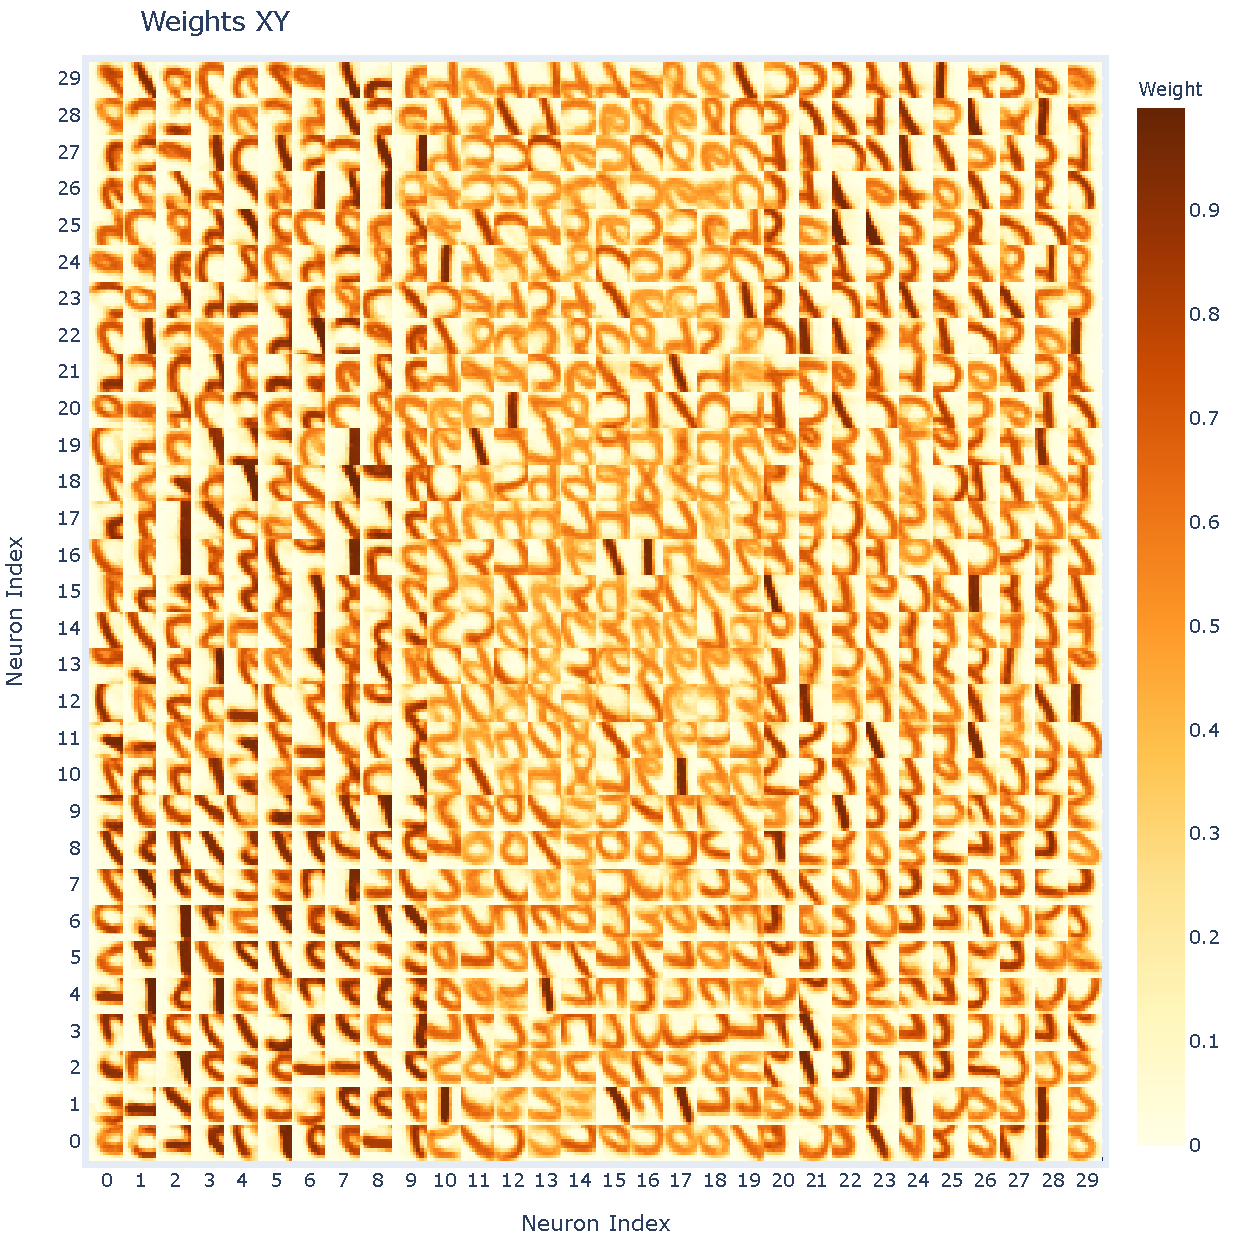
\includegraphics[,
 width=\textwidth,keepaspectratio=true]{weights_XY.pdf}
 \label{weights_XY}
 \caption{Веса XY слоя после обучения}
\end{center}
\end{figure}


\section{Методика}
Во всех экспериментах используются модель интегрирующих нейронов с утечкой. \\ \textbf{Вставить формулу}

\section{Результаты}

\subsection{Сравнение архитектур}
Результаты экспериментов с различными архитектурами

\begin{center}
\begin{tabular}{|l|l|l|l|l|l|l|}
\hline
{Архитектура} & {Фильтры} & {Ядро} & {Веса} & {Нейроны} & {Точность} & {Погрешность}\\
\hline
{LCSNN} & {100} & {12} & {449100} & {900} & {0.8752} & {0.0090}\\
\hline
{LCSNN} & {100} & {8} & {798400} & {1600} & {0.8285} & {0.0021}\\
\hline
{LCSNN} & {25} & {12} & {95400} & {225} & {0.7939} & {0.0038}\\
\hline
{LCSNN} & {25} & {8} & {169600} & {400} & {0.7360} & {0.0103}\\
\hline
{CSNN} & {100} & {8} & {11350} & {1600} & {0.7736} & {0.0188}\\
\hline
{CSNN} & {25} & {12} & {3900} & {225} & {0.6577} & {0.0067}\\
\hline
{CSNN} & {25} & {8} & {1900} & {400} & {0.5807} & {0.0117}\\
\hline
{FCSNN} & {100} & {20} & {44950} & {100} & {0.7340} & {0.0866}\\
\hline
\end{tabular}
\end{center}


\subsection{Обучение конкуренции}
Обучение конкуренции

\section{Заключение}
Было обнаружено, что обучение связей конкуренции нейронов, имеющих общие рецептивные поля, позволяет добиться большей точности распознавания изображений по сравнению с той же архитектурой, но с необучаемыми связями конкуренции. Также было показано, что LCSNN имеет преимущество над CSNN как по скорости обучения, так и по точности распознавания. Таким образом, локально соединенная сеть – перспективная нейросетевая архитектура, превосходящая классические алгоритмы в точности распознавания изображений при обучении без учителя, и подходит для реализации на вычислительном мемристорном нейрочипе.
 
\section{Благодарности}
Благодарности

\printbibliography
\end{document}  
